
%----------------------------------------------------------------------
% SECTION Hardware FPGA

%Themen nach Signalfluss aufbauen
%----------------------------------------------------------------------

\section{Hardware FPGA}
\label{sec:HardwareFPGA}
Das FPGA soll die Umwandlung des Manchestersignals vom MVB, bzw. des Signals
nach dem RS485 Transceiver, in einen Bitstream realisieren. 

Die Konfiguration für das FPGA wurde in der Hardwarebeschreibungssprache VHDL geschrieben. Dabei wurden
mehrere Dateien für die verschiedenen Aufgaben des FPGA erstellt, um eine saubere und simple 
Dateistruktur zu erreichen. Der Code wurde mittels der Designsoftware Quartus geschrieben,
synthetisiert und auf das FPGA geladen.

Der Code ist in fünf Dateien aufgeteilt. Zwar wurde dieser in seine verschiedenen Aufgaben, der
Decodierung des Signals (siehe Kapitel \ref{Manchester Decodierung}), der Ausgabe des Bitstream auf SPI
(siehe Kapitel \ref{fpga:spi}), der Erzeugung der Taktfrequenz für die Abtastung des Manchestersignal,
dem Puffern der Werte nach der Abtastung (siehe Kapitel \ref{fpga:spi}) und zuletzt wurde eine Top-Level Datei erstellt um all diese
Prozesse zu verknüpfen und die Ein- und Ausgänge des FPGA zu konfigurieren.

In Abbildung \ref{fig:AufbauFPGA} sind graphisch in Blockschaltbildern die Verknüpfungen der Dateien zu sehen.

\begin{figure}[H]
    \centering
    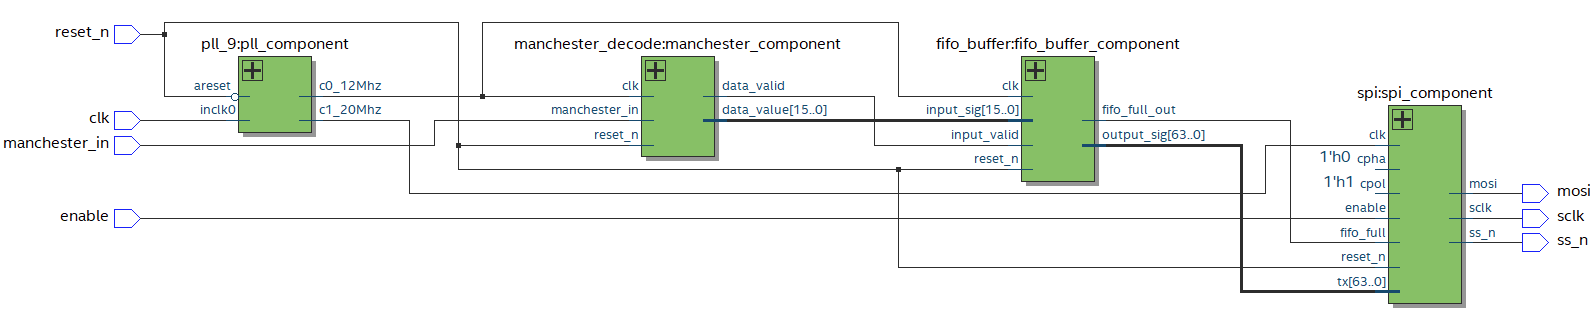
\includegraphics[width=1\linewidth]{Figures/Chap3/FPGA/FPGA_Darstellung_Projekt.png}
    \caption{Aufbau des VHDL-Codes in Blockschaltbildern}
    \label{fig:AufbauFPGA}
\end{figure}

In den folgenden Unterkapiteln werden die einzelnen wichtigsten Prozesse genauer erklärt.\\
\\
Dabei ist wichtig zu erwähnen, dass durch die Decodierung des Manchestersignal, aus einem Bit
(Manchester-Codiert) zwei Bits (Bitstream) werden. Das heisst im 16 Bit grossen 
\textit{data\_value\_reg} ist jeweils ein Byte des MVB abgebildet.\\
\newline
In dieser Arbeit gelten folgende Einheitsnamen und Datengrössen:\\
\textbf{Nutzdatenbyte}\hspace{0.1cm}= \textbf{8 Bit} (Manchester) =\hspace{0.1cm}\textbf{16 Bit} (decodiertes Signal) in \textit{data\_value\_reg}\\
\textbf{Nutzdatenbit}\hspace{0.37cm}= \textbf{1 Bit} (Manchester) =\hspace{0.3cm}\textbf{2  Bit} (decodiertes Signal)
\newpage
\subsection{Manchester Decodierung}
\label{Manchester Decodierung}

Um das Manchestersignal decodieren zu können, muss dieses abgetastet werden. Um möglichst synchron zum
Signal vom MVB zu sein muss die Abtastfrequenz ein Mehrfaches der MVB Bitrate sein. Um die Abtastung möglichst
robust zu machen und Fehler zu vermeiden wurde festgelegt minimal vier mal pro Flanke abzutasten. Somit
wird verhindert dass durch ungewolltes shiften und bei einer Abtastung genau auf dem Flankenwechsel, falsche Werte
decodiert werden.
Bei einer Abtastung von vier mal pro Flanke und somit acht mal pro BT (666 ns = 1.5 MHz) ergibt sich eine Abtastfrequenz von 12 MHz.
Um diese Abtastrate zu realisieren, wurde mit der Designsoftware Quartus eine Taktfrequenz von 12 MHz generiert.
Die abgetasteten Werte werden fortlaufend in ein acht Bit grosses Register \textit{reg\_sample} geschrieben.
In Abbildung \ref{fig:MasterframeAbtastung} ist das Master Start-Delimiter mit den
jeweiligen Abtastpunkten in blau, den Abtastwerten im Register \textit{reg\_sample} von Bit 0 - 7 und den darauffolgenden decodierten 
Werte, welche ins 16 Bit grosse Register \textit{data\_value\_reg} geschrieben werden, zu sehen.
%Immer nach acht Zyklen werden die Daten in diesem Register ausgewertet.

\begin{figure}[H]
    \centering
    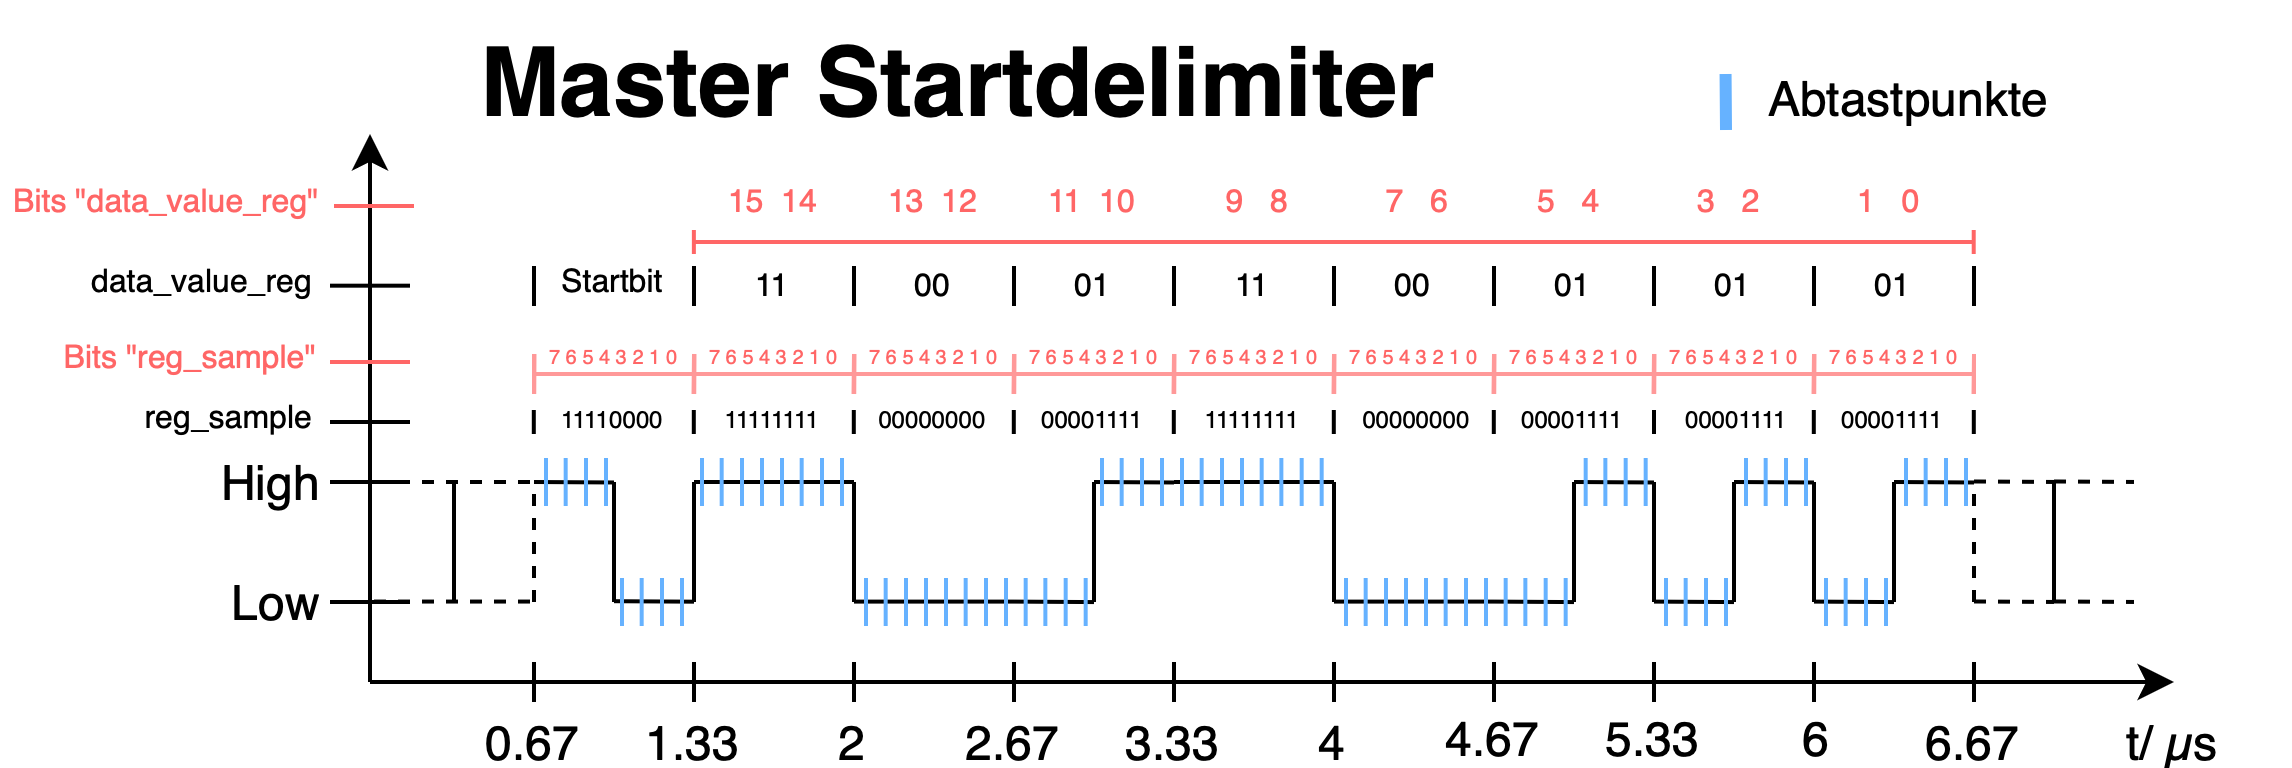
\includegraphics[width=1\linewidth]{Figures/Chap3/FPGA/Abtastpunkte_Master.png}
    \caption{Masterframe Startdelimiter mit Abtastpunkten}
    \label{fig:MasterframeAbtastung}
\end{figure}

\subsubsection{Auswertung Manchestersignal}
\label{Auswertung Manchestersignal}
Immer zu Beginn eines Frame (Master wie auch Slave) wird der Start mit einem Startbit signalisiert, wie dies bereits in Kapitel \ref{sub:StartDelimiter} beschrieben ist.
Sobald das \textit{Start bit} im Auswerteprozess erkannt wird, heisst sobald Bit 5 - 2 im Register \textit{reg\_sample} den Wert \textit{"'1100"'} haben, wechselt das FPGA vom Zustand \textit{IDLE} in den Zustand \textit{RECEIVING}. Dieser Zustandswechsel ist in Abbildung \ref{fig:FPGAIdleRec} dargestellt.

\begin{figure}[H]
    \centering
    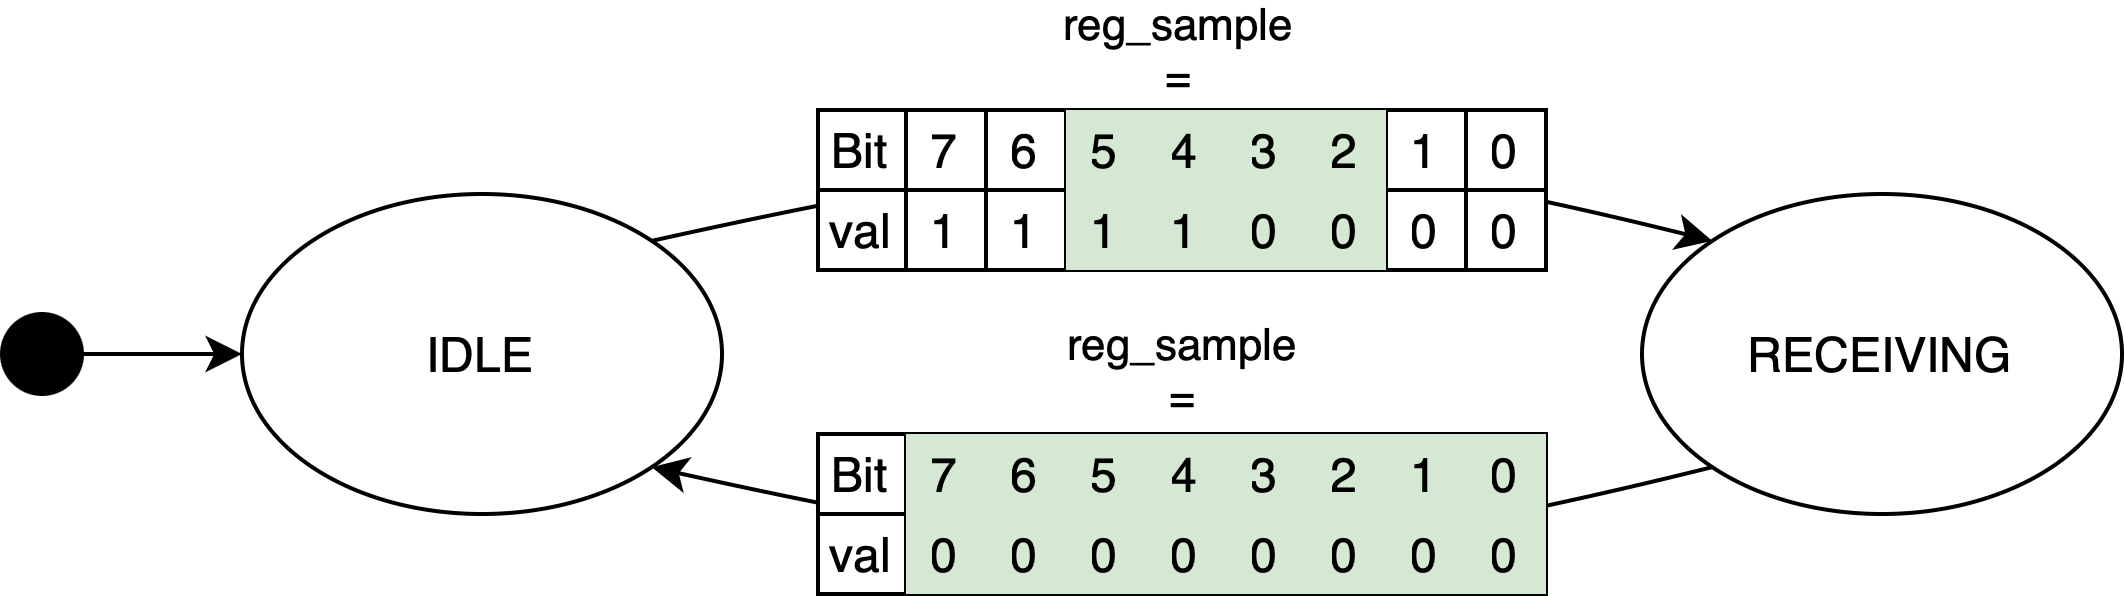
\includegraphics[width=0.7\linewidth]{Figures//Chap3//FPGA/FPGA_idle_rec.png}
    \caption{Zustandsdiagramm FPGA Manchester-Decodierung}
    \label{fig:FPGAIdleRec}
\end{figure}

Im Zustand \textit{RECEIVING} werden Fortlaufend die abgetasteten Werte ins Register 
\textit{reg\_sample} geschrieben und immer nachdem acht mal abgetastet wurde, werden die Daten in diesem Register ausgewertet. Dabei ist im Idealfall immer ein ganzes BT des MVB-Signal im Register abgebildet, was einem Nutzdatenbit entspricht. Idealerweise ist dann auch der Übergang der Flanke von "'0"' auf "'1"' oder von "'1"' auf "'0"' genau bei Bit 4 auf 3 zu sehen. Die Auswertelogik überprüft dann jeweils was an den Stellen 5 - 2 des Registers steht und schreibt dementsprechend die Werte weiter ins Register \textit{data\_value\_reg}. Im Idealfall gibt es dann genau vier Fälle die entstehen können.


% Das sind die folgenden vier:

% \textbf{Fall 1}\\
% Bei einem Übergang von '0' auf '1' beinhaltet \textit{reg\_sample} die Werte \textit{"'00001111"'}. Somit ist bei bit 4 auf 3 der Übergang "'01"' zu sehen. Das ist gleichzeitig der Wert welcher ins \textit{data\_value\_reg} geschrieben wird.

% \textbf{Fall 2}\\
% Bei einem Übergang von '1' auf '0' beinhaltet \textit{reg\_sample} die Werte \textit{"'11110000"'}. Hier ist bei bit 4 auf 3 eine "'10"' zusehen.

% \textbf{Fall 3}\\
% Fall drei deckt die erste violation ab. Heisst wenn das Register nur mit Nullen gefüllt ist \textit{"'00000000"'}. In diesem Fall wird ins \textit{data\_value\_reg} der Wert "'00"' geschrieben.

% \textbf{Fall 4}\\
% Im vierten Fall wird die zweite violation erkannt. Wenn das Register die Werte \textit{"'11111111"'} beinhaltet wird ins \textit{data\_value\_reg} der Wert "'11"' geschrieben.

Da der Abtasttakt nicht synchron mit dem MVB-Takt läuft kann es zu leichten Abweichungen kommen, was dazu führt dass der Flankenwechsel nicht bei Bit 4 auf
3 sondern bei Bit 3 auf 2 oder bei Bit 5 auf 4 zu sehen ist. Um diese weiteren Fälle abzufangen, werden jeweils nicht nur die 
mittleren zwei Bits auf ihre Werte überprüft, sondern gleich die mittleren vier Bits. Somit überprüft der Auswerteprozess das Register nicht nur auf vier, sondern auf acht Fälle.

Da das Register \textit{data\_value\_reg} 16 Werte beinhaltet würde es noch weitere acht Fälle
geben. Das Eintreffen der weiteren Acht Fälle wird durch ein shiften der Bits, wenn das Signal über
drei Auswertezyklen hinweg nicht synchron läuft, verhindert. Somit muss die Auswertelogik Acht
Fälle implementiert haben und diese korrekt abarbeiten.

In Abbildung \ref{fig:FPGAreg_sampleCases} sind alle 16 möglichen Fälle zu 
sehen, welche das Register \textit{data\_value\_reg} annehmen könnte, wenn davon 
ausgegangen wird, dass keine Korrektur durch Shifting implementiert ist und wenn
alle 16 Bits zur Auswertung betrachtet würden.

\begin{figure}[H]
    \centering
    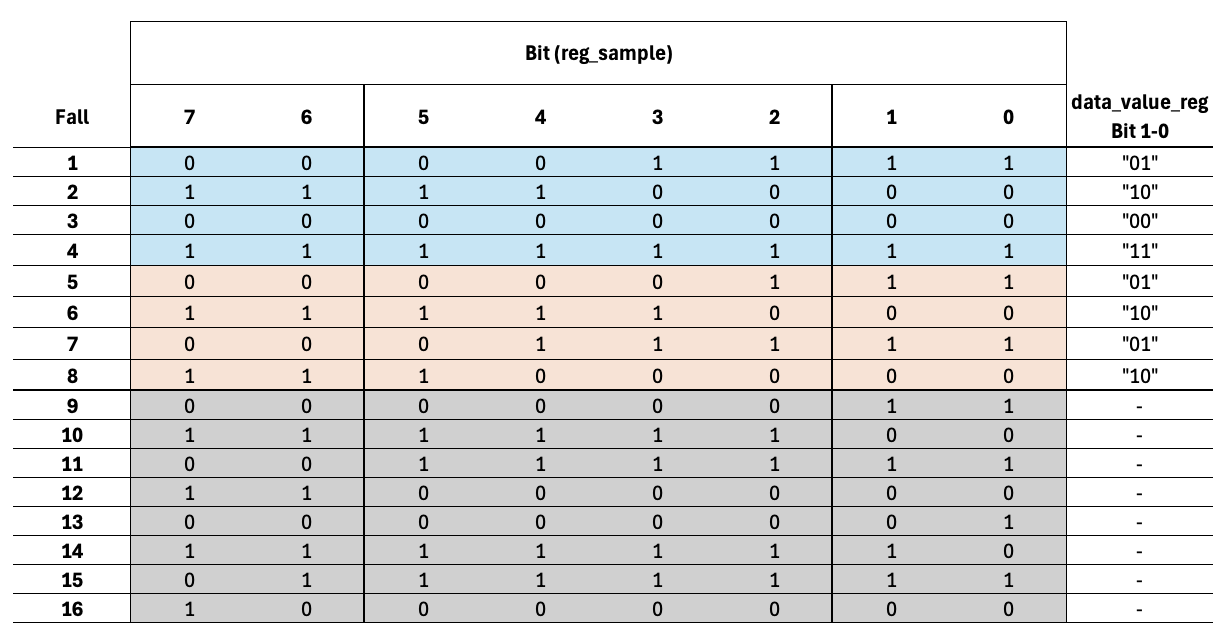
\includegraphics[width=1\linewidth]{Figures//Chap3//FPGA/FPGA_decoding_case.png}
    \caption{Darstellung der Fälle welche das Register \textit{reg\_sample} annehmen kann}
    \label{fig:FPGAreg_sampleCases}
\end{figure}

In Abbildung \ref{fig:FPGAreg_sampleCases} ist zu sehen, dass bei den ersten vier
Fällen genau ein ganzes Nutzdatenbyte im Register abgebildet ist und somit der 
Flankenwechsel bei Bit 4 auf Bit 3 zu sehen ist. In diesen Fällen ist kein 
nachträgliches Shifting nötig und der Wert, welcher in der letzten Spalte zu
sehen ist wird ins \textit{data\_value\_reg} Register geschrieben.

In den Fällen fünf bis acht sind die Werte jeweils um ein Bit verschoben, wodurch
der Flankenwechsel bei Bit 3 auf 2 (Fall 5 \& 6) oder bei Bit 5 auf 4
(Fall 7 \& 8) statt findet. Diese Fälle werden erkannt und die jeweiligen Werte, wie
sie in der letzten Spalte zu sehen sind, ins Register \textit{data\_value\_reg} 
geschrieben.\\
In diesen Fällen notwendig. Dieser Prozess wird in Kapitel \ref{Shifting-Prozess}
erläutert.

In den Fällen neun bis 16 sind die Werte um zwei oder um drei Bits verschoben. Diese Fälle würden dann auftreten, wenn sich das MVB-Signal innerhalb von acht
Abtastungen um zwei ganze Abtastwerte verschiebt. Dies entspricht einer
Verschiebung um 25 \%. In der Norm \textcolor{red}{Norm referenzieren} ist
festgehalten dass eine maximale Abweichung zur Taktfrequenz 1.5 MHz um 0.01 \% vorkommen kann.\\
Daher werden die Fälle 9 bis 16 nie erreicht und müssen nicht in der Auswertelogik
implementiert sein.
 
%  Folgend die Fälle fünf bis acht:

% \textbf{Fall 5}\\
% Ist durch eine Verschiebung nun der Übergang von Bit 5 auf 4 zu sehen, heisst beinhaltet das Register \textit{reg\_sample} die Werte \textit{"'00011110"'}, wird das erkannt und es wird gleichermasen ein "'01"' ins \textit{data\_value\_reg} geschrieben.

% \textbf{Fall 6}\\
% Bei Fall sechs ist der übergang wieder am gleichen Ort wie bei Fall fünf. Nun aber wird eine "'10"' erkannt und ins \textit{data\_value\_reg} geschrieben.

% \textbf{Fall 7}\\
% Im siebten Fall ist der Übergang nun bei Bit 3 auf 2. Es ergibt sich das Register \textit{reg\_sample} welches die Werte \textit{"'01111000"'} beinhaltet und somit den Wert "'01"' schreibt.

% \textbf{Fall 8}\\
% Im letzten Fall ist der Übergang wieder am gleichen Ort wie in Fall sieben, aber nun wird ein "'10"' erkannt und dann auch ins Register \textit{data\_value\_reg} geschrieben.

% Trifft bei der Auswertung einer der Fälle 5 - 8 zu, so wird entweder die Variable \textit{shift\_up} oder \textit{shift\_down} auf '1' gesetzt und weiter an den Prozess \textit{shifting} übergeben, welcher die Abweichung aktiv korrigiert.

Die erläuterte Auswertelogik ist unten, in VHDL implementiert, zu sehen:

\begin{lstlisting}[language=vhdl]
decode_proc: PROCESS (clk, reset_n)
BEGIN		
    IF(reset_n = '0') THEN
       data_value_reg <= (others => '0');
       shift_up <= '0';
       shift_down <= '0';	
    ELSIF(rising_edge(clk)) THEN
       shift_up <= '0';
       shift_down <= '0';
       IF state = RECEIVING THEN
    	   IF count_sample = 0 THEN
    	      data_value_reg(15 DOWNTO 2) <= data_value_reg(13 DOWNTO 0);
    	      IF reg_sample(5 DOWNTO 2) = "0011" THEN
    	         data_value_reg(1 DOWNTO 0) <= "01";
    	      ELSIF reg_sample(5 DOWNTO 2) = "1100" THEN
    	         data_value_reg(1 DOWNTO 0) <= "10";
    	      ELSIF reg_sample(5 DOWNTO 2) = "0001" THEN
    	         data_value_reg(1 DOWNTO 0) <= "01";
    	         shift_up <= '1';
    	      ELSIF reg_sample(5 DOWNTO 2) = "1110" THEN
    	         data_value_reg(1 DOWNTO 0) <= "10";
    	         shift_up <= '1';
    	      ELSIF reg_sample(5 DOWNTO 2) = "0111" THEN
    	         data_value_reg(1 DOWNTO 0) <= "01";
    	         shift_down <= '1';
    	      ELSIF reg_sample(5 DOWNTO 2) = "1000" THEN
    	         data_value_reg(1 DOWNTO 0) <= "10";
    	         shift_down <= '1';
    	      ELSIF reg_sample(5 DOWNTO 2) = "0000" THEN
    	         data_value_reg(1 DOWNTO 0) <= "00";
    	      ELSIF reg_sample(5 DOWNTO 2) = "1111" THEN
    	         data_value_reg(1 DOWNTO 0) <= "11";
              END IF;
    	   END IF;
       END IF;		
    END IF;
END PROCESS;
\end{lstlisting}

\newpage

\subsubsection{Shifting-Prozess}
\label{Shifting-Prozess}
Wie in Kapitel \ref{Manchester Decodierung} erwähnt, müssen in einigen Fälle mehr oder weniger
Werte ins Register \textit{reg\_sample} geschrieben werden. Diese Aufgabe wird in einem
separaten Prozess abgearbeitet. Es wird geprüft wie oft \textit{shift\_up} in Fall 5 \& 6 bzw. \textit{shift\_down} in Fall 7 \& 8 auf '1' gesetzt wurde.
In Abbildung \ref{fig:FPGAShiftingCases} sind die Fälle bei denen ein Shifting notwendig ist
zu sehen. In grün eingefärbt ist zu sehen wann \textit{shift\_up} und \textit{shift\_down}
gesetzt werden und in welche Richtung \textit{count\_shift} zählt.

\begin{figure}[H]
    \centering
    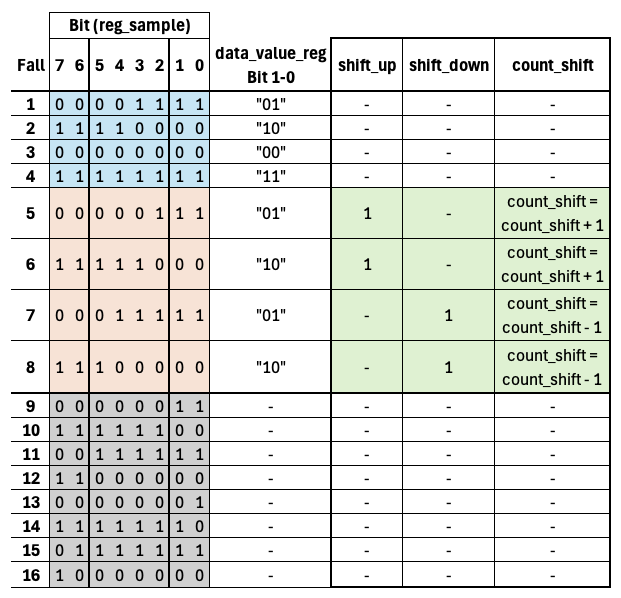
\includegraphics[width=0.9\linewidth]{Figures//Chap3//FPGA/FPGA_Shifting.png}
    \caption{Fälle in denen ein Shifting der Bits notwendig ist}
    \label{fig:FPGAShiftingCases}
\end{figure}

% Dies geschieht mit einem counter \textit{count\_shift}, welcher im Falle \textit{shift\_up} den Zählerwert um eins erhöht und im Falle \textit{shift\_down} um eins reduziert.
Sobald \textit{count\_shift} den Wert "'2"' drei mal übersteigt so wird das Register \textit{reg\_sample} das nächste mal nicht nach acht, sondern nach sieben mal ausgewertet. Falls der Zählerwert, ebenfalls drei mal, den Wert "'-2"' unterbietet so wird die nächste Auswertung der Werte nach neun Abtastwerten statt finden. Mit dieser Logik wird aktiv überprüft ob der Flankenwechsel immer in der Mitte des \textit{reg\_sample} Registers zu erkennen ist und falls dies drei mal hintereinander nicht der Fall ist, so wird reagiert und ein Bit mehr oder weniger ins Register geschrieben.
Nach der Korrektur wird der Counter \textit{count\_shift} wieder auf '0' gesetzt. Es wird
erst nach drei mal reagiert, um somit zu verhindern dass die Logik bei einer einmaligen 
Abweichung durch falsches shiften die Abweichung noch grösser macht und sich somit sehr oft
selbst korrigieren muss.

\newpage
Die Implementierung des Shifting-Prozess in VHDL ist folglich zu sehen:

\begin{lstlisting}[language=vhdl]
shift_proc: PROCESS (clk, reset_n)
BEGIN		
	IF(reset_n = '0') THEN
		samples_per_bit <= to_unsigned(7, 4);
		count_shift <= (others => '0');
	ELSIF(rising_edge(clk)) THEN
		IF state = IDLE THEN
			samples_per_bit <= to_unsigned(7, 4);
			count_shift <= (others => '0');
		ELSE	
			IF shift_up = '1' THEN
				count_shift <= count_shift + 1;
			ELSIF shift_down = '1' THEN
				count_shift <= count_shift - 1;
			END IF;
			IF count_shift > 2 THEN
				samples_per_bit <= to_unsigned(8, 4);
				count_shift <= (others => '0');
			ELSIF count_shift < -2 THEN
				samples_per_bit <= to_unsigned(6, 4);
				count_shift <= (others => '0');
			END IF;
			IF count_sample = 0 THEN
				samples_per_bit <= to_unsigned(7, 4);
			END IF;	
		END IF;
	END IF;
END PROCESS;
\end{lstlisting}

\subsection{SPI}
\label{fpga:spi}
Damit die Daten aus dem Register \textit{data\_value\_reg} für die weitere Auswertung und Verarbeitung an den Mikrocontroller ESP32 übertragen werden können, wurde das Übertragungsprotokoll SPI implementiert.\\
\\
Als Basis zum VHDL-Code wurde die bereits geschriebene SPI-Master Implementierung von Github genommen und angepasst.
Der bereits geschriebene Code ist unter dem Link \href{https://github.com/nematoli/SPI-FPGA-VHDL/blob/master/hdl/spi_master.vhd}{\textit{https://github.com/nematoli/SPI-FPGA-VHDL/blob/master/hdl/spi\_master.vhd}} \\zu finden.


Es wurde festgelegt, dass das FPGA als Master und der ESP32 als Slave agiert. Als Modi wurden \textit{CPOL=0} und \textit{CPHA=0} bestimmt. Die Übertragungsfrequenz wurde möglichst hoch gewählt, damit die Daten sicherlich schneller übertragen, als die neu abgetasteten Werte wieder ins Register geschrieben, werden.
Das FPGA sowohl als auch der ESP32 mussten die Frequenz erreichen können. Schlussendlich wurde 20 MHz als Übertragungsrate festgelegt.

Werden immer, sobald das Register \textit{data\_value\_reg} voll ist, die Daten auf das SPI übertragen, so würden alle \textit{5.33 µs} neue Daten übertragen werden. Die Zahl berechnet sich folgendermassen:
% Requires: \usepackage{siunitx}

\begin{equation}
    8 \, \text{Nutzdatenbit} \times 666 \, \text  ns = 5328 \, \text  ns = 5.33  \mu\text  s \label{eq:calc_Nutzdatenbit1}
\end{equation}
\textcolor{red}{Abstand zu Einheiten weiss nicht wie einfügen}

Da der ESP32 nur alle \textit{16 µs} neue Daten empfangen kann (siehe Kapitel \ref{sec:ResultatESP32}) wurde entschieden, dass das FPGA die Daten jeweils puffert und sobald der Puffer von 32 Nutzdatenbits voll ist, diesen auf das SPI überträgt. Damit ergibt sich folgende Zeit zwischen den Übertragungen:

\begin{equation}
    32 \, \text{Nutzdatenbit} \times 666 \, \text ns = 21312 \, \text ns = 21.3  \mu\text s \label{eq:calc_Nutzdatenbit2}
\end{equation}
\textcolor{red}{Abstand zu Einheiten weiss nicht wie einfügen}

Unterhalb ist die Logik für das Schreiben des Puffers in VHDL zu sehen:
\begin{lstlisting}[language=vhdl]
PROCESS(clk, reset_n)
BEGIN
    IF reset_n = '0' THEN
        fifo <= (others => (others => '0'));
        write_ptr <= 0;
        fifo_full <= '0';
        buffer_ready <= '0';
        output_sig <= (others => '0');
    ELSIF rising_edge(clk) THEN
        IF input_valid = '1' and fifo_full = '0' THEN
            fifo(write_ptr) <= input_sig;
            write_ptr <= write_ptr + 1
            IF write_ptr = 3 THEN
                fifo_full <= '1';
                buffer_ready <= '1';
            ELSE
                buffer_ready <= '0';
            END IF;
        END IF;
        IF fifo_full = '1' THEN
            output_sig <= fifo(0) & fifo(1) & fifo(2) & fifo(3);
            fifo_full <= '0';
            write_ptr <= 0;
        END IF;
    END IF;
END PROCESS;
\end{lstlisting}

Wodurch der ESP32 genug Zeit für die Verarbeitung hat und somit alle Daten korrekt und ohne Verlust übertragen werden können.